% \documentclass{article}
\documentclass[../../outputs/main.tex]{subfiles}

% Any packages or configurations specific to this section
\usepackage{lipsum}
\usepackage{graphicx}

\begin{document}

\section{Case Study Demonstration}
% The energy price data is taken from the ComEd hourly live prices data \cite{comedLivePrices} for 10 November 2023. 

\subsection{Simulation Data: IEEE 123 Bus Test System}

\begin{figure}[h!]
    \centering
    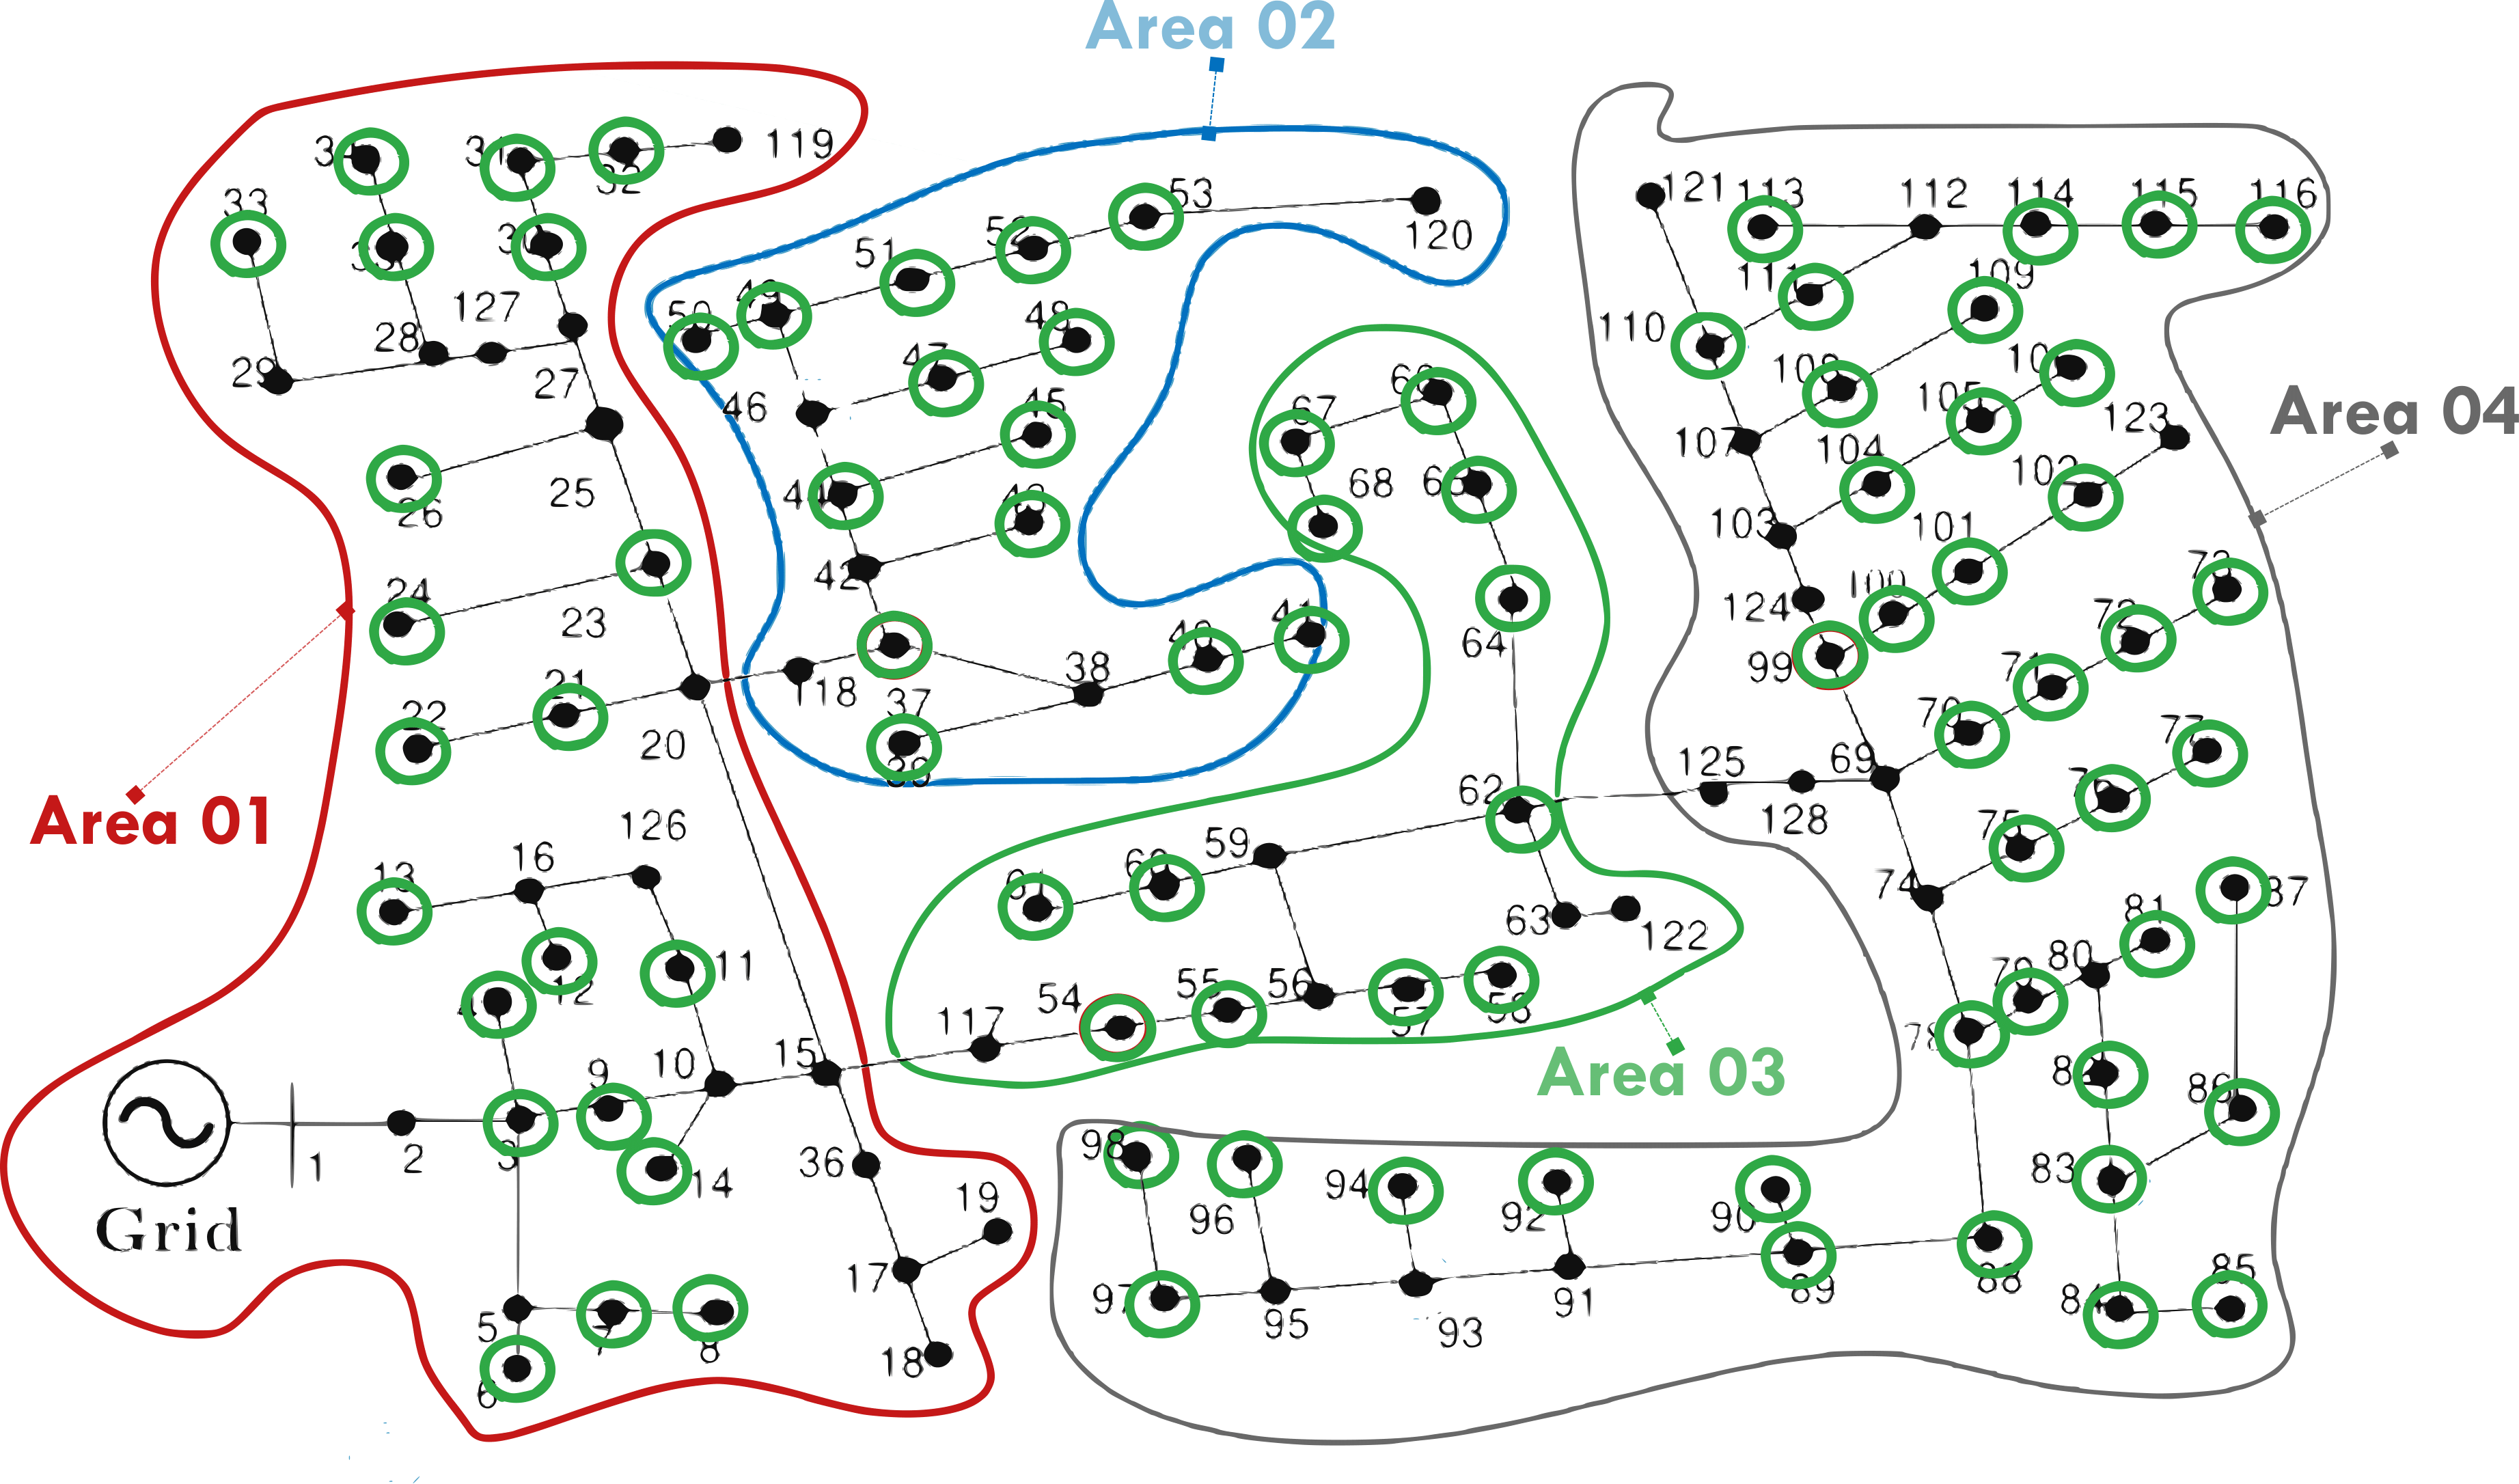
\includegraphics[width=\linewidth]{../figures/ieee123-FourAreas.png}
    \caption{IEEE 123 Node System Divided Into Four Areas}
    \label{fig:ieee123-four-area-figure}
\end{figure}

\textcolor{red}{Change figure to display battery buses and PV buses}

\begin{figure}[h!]
    \centering
    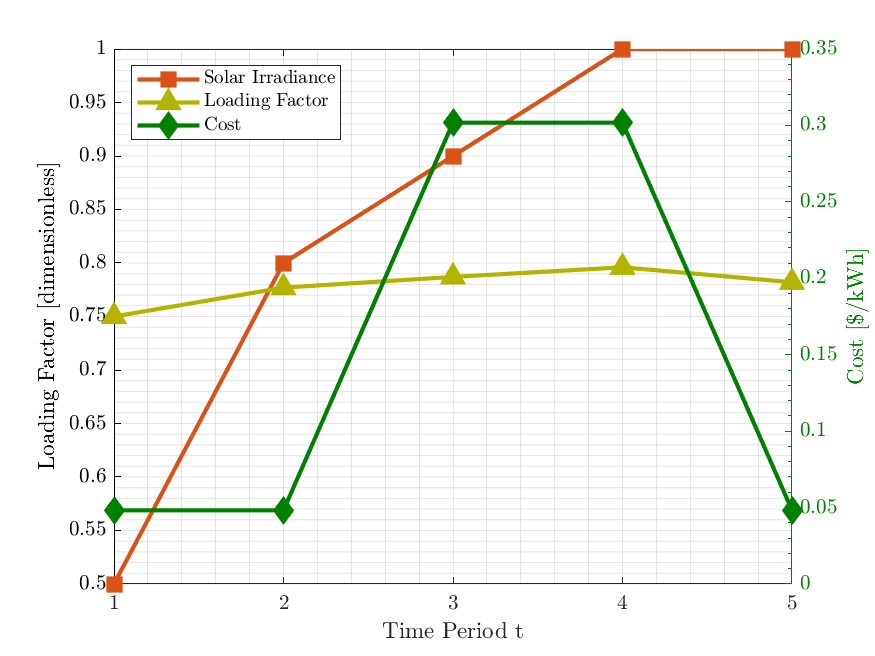
\includegraphics[height=0.25\textheight]{../figures/T5-inputCurves/InputCurves_Horizon_5.png}
    \caption{Forecasts for Demand Power, Irradiance and Cost of Substation Power over a 5 Hour Horizon}
    \label{fig:inputCurve-5}
\end{figure}


% \begin{table}[h!]
%     \centering
%     \caption{Parameter Values}
%     \begin{tabular}{|l|c|}
%     \hline
%     \textbf{Parameter} & \textbf{Value} \\ \hline
%     $V_{min}, V_{max}$ & 0.95, 1.05 \\ \hline
%     $p_{D_{R_j}}$ & $0.33 p_{L_{R_j}}$ \\ \hline
%     $S_{D_{R_j}}$ & $1.2 p_{D_{R_j}}$ \\ \hline
%     $P_{B_{R_j}}$ & $0.33 p_{L_{R_j}}$ \\ \hline
%     $B_{R_j}$ & $T_{fullCharge} \times p_{B_{R_j}}$ \\ \hline
%     $T_{fullCharge}$ & 4 h \\ \hline
%     $\Delta t$ & 1 h \\ \hline
%     $\eta_C, \eta_D$ & 0.95, 0.95 \\ \hline
%     $soc_{min}, soc_{max}$ & 0.30, 0.95 \\ \hline
%     $\alpha$ & 0.001 \\ \hline
%     \end{tabular}
%     \label{table:parameter-values}
% \end{table}
% \begin{table}[h!]
%     \centering
%     \caption{Parameter Values}
%     \begin{tabular}{|l|c|}
%     \hline
%     \textbf{Parameter} & \textbf{Value} \\ \hline
%     $V_{min}, V_{max}$ & 0.95, 1.05 \\ \hline
%     $p_{D_{R_j}}$ & $0.33 p_{L_{R_j}}$ \\ \hline
%     $S_{D_{R_j}}$ & $1.2 p_{D_{R_j}}$ \\ \hline
%     $P_{B_{R_j}}$ & $0.33 p_{L_{R_j}}$ \\ \hline
%     $B_{R_j}$ & $T_{fullCharge} \times p_{B_{R_j}}$ \\ \hline
%     $T_{fullCharge}$ & 4 h \\ \hline
%     $\Delta t$ & 1 h \\ \hline
%     $\eta_C, \eta_D$ & 0.95, 0.95 \\ \hline
%     $soc_{min}, soc_{max}$ & 0.30, 0.95 \\ \hline
%     $\alpha$ & 0.001 \\ \hline
%     \end{tabular}
%     \label{table:parameter-values}
% \end{table}

\def\ds{\rule{0pt}{1.5ex}} % this will lower the subscript by that amount, useful for $p_{D_{R_j}}$ where otherwise p and D appear to be almost at the same level.

\begin{table}[h!]
    \centering
    \caption{Parameter Values}
    \begin{tabular}{|l|c|}
    \hline
    \textbf{Parameter} & \textbf{Value} \\ \hline
    $V_{min}, V_{max}$ & 0.95, 1.05 \\ \hline
    $p_{\ds D_{R_j}}$ & $0.33 p_{\ds L_{R_j}}$ \\ \hline
    $S_{D_{R_j}}$ & $1.2 p_{\ds D_{R_j}}$ \\ \hline
    $P_{B_{R_j}}$ & $0.33 p_{\ds L_{R_j}}$ \\ \hline
    $B_{R_j}$ & $T_{fullCharge} \times P_{B_{R_j}}$ \\ \hline
    $T_{fullCharge}$ & 4 h \\ \hline
    $\Delta t$ & 1 h \\ \hline
    $\eta_C, \eta_D$ & 0.95, 0.95 \\ \hline
    $soc_{min}, soc_{max}$ & 0.30, 0.95 \\ \hline
    $\alpha$ & 0.001 \\ \hline
    \end{tabular}
    \label{table:parameter-values}
\end{table}


\end{document}
